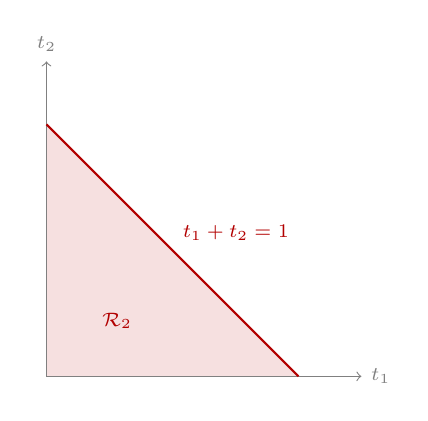
\begin{tikzpicture}[x=3.2cm,y=3.2cm]
\fill[red!70!black!12] (0,0)--(1,0)--(0,1)--cycle;
\draw[black!50,->] (0,0)--(1.25,0) node[right,font=\scriptsize] {$t_1$};
\draw[black!50,->] (0,0)--(0,1.25) node[above,font=\scriptsize] {$t_2$};
\draw[red!70!black,thick] (1,0)--(0,1) node[midway,above right,font=\scriptsize] {$t_1+t_2=1$};
\node[font=\scriptsize,red!70!black] at (0.28,0.22) {$\mathcal R_2$};
\end{tikzpicture}
